\documentclass[usenames, dvipsnames, aspectratio=169]{beamer}

%%%%%
%%%%%
%%%%%
%%%%%
%%%%%

\usepackage{xcolor}
\usepackage{tikz}
\usetikzlibrary{backgrounds}
\usetikzlibrary{arrows, shapes}
\usetikzlibrary{tikzmark}
\usetikzlibrary{calc}
\usetikzlibrary{positioning}
\usetikzlibrary{shadows}
\usetikzlibrary{trees, mindmap}
\usetikzlibrary{lindenmayersystems}

\usepackage{pgfplots}
\pgfplotsset{compat=newest}

\usepackage{tcolorbox}

\newcommand{\highlight}[2]{\colorbox{#1!17}{$\displaystyle #2$}}
\newcommand{\highlightdark}[2]{\colorbox{#1!47}{$\displaystyle #2$}}
\renewcommand{\highlight}[2]{\colorbox{#1!17}{#2}}
\renewcommand{\highlightdark}[2]{\colorbox{#1!47}{#2}}

\usepackage[utf8]{inputenc}
\usepackage[english]{babel}

\usepackage{amsmath, amssymb, amsfonts}

\usepackage[]{bm}
\usepackage[]{nicefrac}

\usepackage{graphicx}
\usepackage{multimedia}

\usepackage{xspace}

\newcommand{\lap}{\nabla^2}

%%%%%
%%%%%
%%%%%
%%%%%
%%%%%





\usetheme{default}
\usefonttheme{professionalfonts}
\setbeamertemplate{navigation symbols}{}
\setbeamertemplate{itemize items}[circle]
\setbeamercolor{itemize item}{fg=white}

\setbeamerfont{title}{series=\bfseries, size=\normalfont\Large}
\setbeamercolor{title}{fg=white}

\setbeamerfont{author}{size=\normalfont\small}
\setbeamercolor{author}{fg=white}

\setbeamerfont{frametitle}{series=\bfseries, size=\normalfont}
\setbeamercolor{frametitle}{fg=white}

\setbeamerfont{framesubtitle}{size=\normalfont\large}
\setbeamercolor{framesubtitle}{fg=white}

\setbeamercolor{background canvas}{bg=black}
\setbeamercolor{normal text}{fg=white}

\setbeamercolor{local structure}{fg=white}





\graphicspath{{imgs/}}




%%%%%
%%%%%
%%%%%
%%%%%
%%%%%

\pgfdeclarelindenmayersystem{Koch curve}{
  \symbol{X}{\pgflsystemdrawforward}
  \rule{X -> X + X -- X + X}
}

\pgfdeclarelindenmayersystem{Three Half curve}{
  \symbol{X}{\pgflsystemdrawforward}
  \rule{X -> X + X - X - XX + X + X - X}
}

\pgfdeclarelindenmayersystem{Sierpinsky}{
  \symbol{X}{\pgflsystemdrawforward}
  \symbol{Y}{\pgflsystemdrawforward}
  \rule{X -> Y - X - Y}
  \rule{ Y -> X + Y + X}
}

\pgfdeclarelindenmayersystem{Hilbert curve}{
  \rule{L -> +RF-LFL-FR+}
  \rule{R -> -LF+RFR+FL-}
}

\pgfdeclarelindenmayersystem{Cantor set}{
  \rule{F -> FfF}
  \rule{f -> fff}
}


\title{Strange Attractors}
\author{Jean-Christophe LOISEAU}
\institute{Arts \& Métiers Institute of Technology, January 2022}
\date{}

\begin{document}

\frame{\titlepage}

{
  \setbeamercolor{background canvas}{bg=white}
  \setbeamercolor{background canvas}{bg=white}
  \setbeamercolor{normal text}{fg=black}

  \usebeamercolor[fg]{normal text}

  \setbeamercolor{frametitle}{fg=black}
  \setbeamercolor{framesubtitle}{fg=black}
  \setbeamercolor{itemize item}{fg=black}

  \begin{frame}[t, c]{Lorenz system}{}
    \vfill
    \centering
    \large

    \begin{minipage}{.48\textwidth}
      \centering
      \begin{tikzpicture}
        \begin{axis}[
            xmin=-25, xmax=25,
            ymin=0, ymax=50,
            height=.75\textheight,
            hide axis
          ]
          \addplot[smooth, very thin, black, opacity=0.75] table[x=x, y=z]{data/lorenz_attractor.dat};
        \end{axis}
      \end{tikzpicture}
    \end{minipage}%
    \hfill
    \begin{minipage}{.48\textwidth}
      \centering
      \begin{tikzpicture}[>=stealth]
        \begin{axis}[
            xmin=30, xmax=48,
            ymin=30, ymax=48,
            xlabel={$z_k$}, ylabel={$z_{k+1}$},
            width=.8\textwidth,
            height=.8\textwidth,
            axis lines = middle,
            axis line style = {->},
            x label style={at={(axis description cs:1, 0)}, anchor=north},
            y label style={at={(axis description cs:0, 1)}, anchor=west},
            ytick style={draw=none},
            yticklabels=\empty,
            xtick style={draw=none},
            xticklabels=\empty,
          ]

          \addplot[only marks, orange, mark size=0.5pt] table[x=x, y=y]{data/lorenz_map.dat};

          \draw[black, thin] (axis cs:30, 30) -- (axis cs:45, 45) node[] {};
        \end{axis}
      \end{tikzpicture}      
    \end{minipage}

    \vfill
  \end{frame}

  \begin{frame}[t, c]{R\"ossler system}{}
    \vfill
    \centering
    \large

    \begin{minipage}{.48\textwidth}
      \centering
      \includegraphics[width=.8\textwidth]{rossler_system}
    \end{minipage}%
    \hfill
    \begin{minipage}{.48\textwidth}
      \begin{tikzpicture}[>=stealth]
        \begin{axis}[
            xmin=0, xmax=8,
            ymin=0, ymax=8,
            xlabel={$y_k$}, ylabel={$y_{k+1}$},
            width=.8\textwidth,
            height=.8\textwidth,
            axis lines = middle,
            axis line style = {->},
            x label style={at={(axis description cs:1, 0)}, anchor=north},
            y label style={at={(axis description cs:0, 1)}, anchor=west},
            ytick style={draw=none},
            yticklabels=\empty,
            xtick style={draw=none},
            xticklabels=\empty,
          ]

          \addplot[only marks, orange, mark size=0.5pt] table[x=x, y=y]{data/rossler_map.dat};

          \draw[black, thin] (axis cs:0, 0) -- (axis cs:8, 8) node[] {};
        \end{axis}
      \end{tikzpicture}            
    \end{minipage}

    \vfill
  \end{frame}

}

\begin{frame}[t, c]{Making pastry}{}
  \vfill
  \large

  \begin{minipage}{.48\textwidth}
    \centering
    \includegraphics[width=\textwidth]{puff_pastry}
  \end{minipage}%
  \hfill
  \begin{minipage}{.48\textwidth}
    A lot can be understood about strange attractors by looking at how puff pastry is being made.
  \end{minipage}

  \vfill
\end{frame}

\begin{frame}[t, c]{Baker's map}{}
  \vfill
  \large

  \[
  \left(x_{k+1}, y_{k+1} \right)
  =
  \begin{cases}
    \left(2 x_k, a y_k \right) \quad \textrm{for } 0 \leq x_k \leq \dfrac{1}{2} \\
    \\
    \left(2 x_k - 1, ay_k + 1 - a \right) \quad \textrm{for } \dfrac{1}{2} \leq x_k \leq 1.
  \end{cases}
  \]

  \vfill
\end{frame}

{
  \setbeamercolor{background canvas}{bg=white}
  \setbeamercolor{background canvas}{bg=white}
  \setbeamercolor{normal text}{fg=black}

  \usebeamercolor[fg]{normal text}
  
  \setbeamercolor{frametitle}{fg=black}
  \setbeamercolor{framesubtitle}{fg=black}
  \setbeamercolor{itemize item}{fg=black}
  
  \begin{frame}[t, c]{Baker's map ($a = \dfrac{1}{2}$)}{}
    \centering
    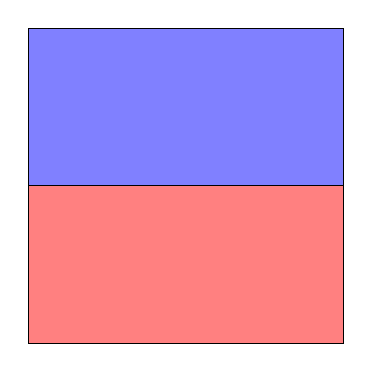
\begin{tikzpicture}
      \draw[fill=red!50] (0, 0) rectangle (4, 2);
      \draw[fill=blue!50] (0, 2) rectangle (4, 4);
    \end{tikzpicture}
  \end{frame}
  
  \begin{frame}[t, c]{Baker's map ($a = \dfrac{1}{2}$)}{}
    \centering
    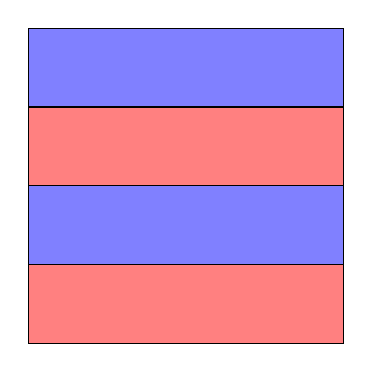
\begin{tikzpicture}
      \draw[fill=red!50] (0, 0) rectangle (4, 1);
      \draw[fill=blue!50] (0, 1) rectangle (4, 2);
      
      \draw[fill=red!50] (0, 2) rectangle (4, 3);
      \draw[fill=blue!50] (0, 3) rectangle (4, 4);
    \end{tikzpicture}
  \end{frame}

  \begin{frame}[t, c]{Baker's map ($a = \dfrac{1}{2}$)}{}
    \centering
    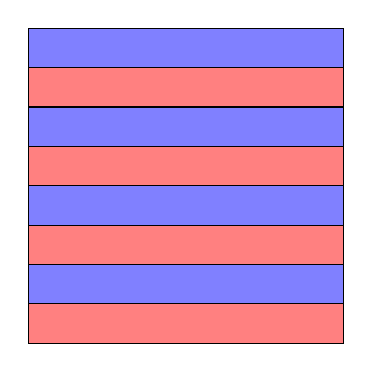
\begin{tikzpicture}
      \draw[fill=red!50] (0, 0) rectangle (4, 0.5);
      \draw[fill=blue!50] (0, 0.5) rectangle (4, 1);
      
      \draw[fill=red!50] (0, 1) rectangle (4, 1.5);
      \draw[fill=blue!50] (0, 1.5) rectangle (4, 2);

      \draw[fill=red!50] (0, 2) rectangle (4, 2.5);
      \draw[fill=blue!50] (0, 2.5) rectangle (4, 3);
      
      \draw[fill=red!50] (0, 3) rectangle (4, 3.5);
      \draw[fill=blue!50] (0, 3.5) rectangle (4, 4);

    \end{tikzpicture}
  \end{frame}

  \begin{frame}[t, c]{Baker's map ($a = \dfrac{1}{2}$)}{}
    \centering
    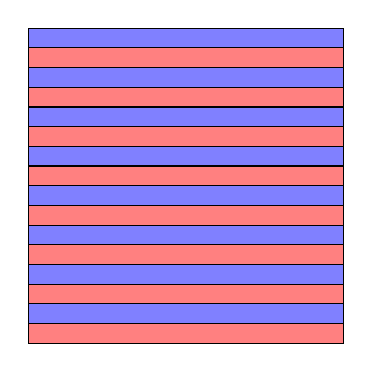
\begin{tikzpicture}
      \draw[fill=red!50] (0, 0) rectangle (4, 0.25);
      \draw[fill=blue!50] (0, 0.25) rectangle (4, 0.5);
      
      \draw[fill=red!50] (0, 0.5) rectangle (4, 0.75);
      \draw[fill=blue!50] (0, 0.75) rectangle (4, 1);

      \draw[fill=red!50] (0, 1) rectangle (4, 1.25);
      \draw[fill=blue!50] (0, 1.25) rectangle (4, 1.5);
      
      \draw[fill=red!50] (0, 1.5) rectangle (4, 1.75);
      \draw[fill=blue!50] (0, 1.75) rectangle (4, 2);

      \draw[fill=red!50] (0, 2) rectangle (4, 2.25);
      \draw[fill=blue!50] (0, 2.25) rectangle (4, 2.5);
      
      \draw[fill=red!50] (0, 2.5) rectangle (4, 2.75);
      \draw[fill=blue!50] (0, 2.75) rectangle (4, 3);

      \draw[fill=red!50] (0, 3) rectangle (4, 3.25);
      \draw[fill=blue!50] (0, 3.25) rectangle (4, 3.5);
      
      \draw[fill=red!50] (0, 3.5) rectangle (4, 3.75);
      \draw[fill=blue!50] (0, 3.75) rectangle (4, 4);

    \end{tikzpicture}
  \end{frame}

}

\begin{frame}[t, c]{Baker's map ($a = \dfrac{1}{2}$)}{}
  \vfill
  \large
  \begin{minipage}{.38\textwidth}
    \centering
    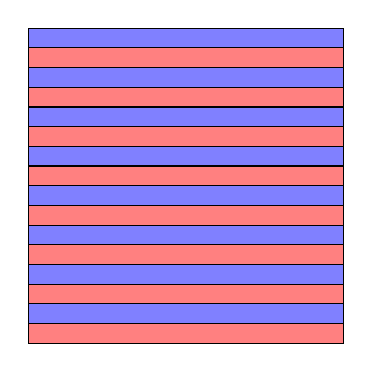
\begin{tikzpicture}
      \draw[fill=red!50] (0, 0) rectangle (4, 0.25);
      \draw[fill=blue!50] (0, 0.25) rectangle (4, 0.5);
      
      \draw[fill=red!50] (0, 0.5) rectangle (4, 0.75);
      \draw[fill=blue!50] (0, 0.75) rectangle (4, 1);

      \draw[fill=red!50] (0, 1) rectangle (4, 1.25);
      \draw[fill=blue!50] (0, 1.25) rectangle (4, 1.5);
      
      \draw[fill=red!50] (0, 1.5) rectangle (4, 1.75);
      \draw[fill=blue!50] (0, 1.75) rectangle (4, 2);

      \draw[fill=red!50] (0, 2) rectangle (4, 2.25);
      \draw[fill=blue!50] (0, 2.25) rectangle (4, 2.5);
      
      \draw[fill=red!50] (0, 2.5) rectangle (4, 2.75);
      \draw[fill=blue!50] (0, 2.75) rectangle (4, 3);

      \draw[fill=red!50] (0, 3) rectangle (4, 3.25);
      \draw[fill=blue!50] (0, 3.25) rectangle (4, 3.5);
      
      \draw[fill=red!50] (0, 3.5) rectangle (4, 3.75);
      \draw[fill=blue!50] (0, 3.75) rectangle (4, 4);

    \end{tikzpicture}
  \end{minipage}%
  \hfill
  \begin{minipage}{.58\textwidth}
    For $a = \nicefrac{1}{2}$, Baker's map is \textbf{\alert{area-preserving}}

    \[
    \textrm{area} \left( \mathcal{B}(R) \right) = \textrm{area}\left(R\right).
    \]

    \medskip

    The square $S$ is mapped \emph{onto} itself and transients never die.
    Orbits never settle down to a lower-dimensional attractor.
  \end{minipage}
  \vfill
\end{frame}


\begin{frame}[t, c]{Baker's map ($a = \dfrac{1}{2}$)}{}
  \vfill
  \large
  \begin{minipage}{.38\textwidth}
    \centering
    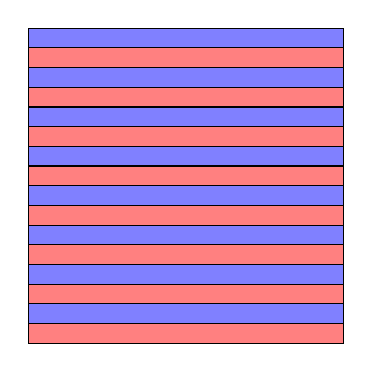
\begin{tikzpicture}
      \draw[fill=red!50] (0, 0) rectangle (4, 0.25);
      \draw[fill=blue!50] (0, 0.25) rectangle (4, 0.5);
      
      \draw[fill=red!50] (0, 0.5) rectangle (4, 0.75);
      \draw[fill=blue!50] (0, 0.75) rectangle (4, 1);

      \draw[fill=red!50] (0, 1) rectangle (4, 1.25);
      \draw[fill=blue!50] (0, 1.25) rectangle (4, 1.5);
      
      \draw[fill=red!50] (0, 1.5) rectangle (4, 1.75);
      \draw[fill=blue!50] (0, 1.75) rectangle (4, 2);

      \draw[fill=red!50] (0, 2) rectangle (4, 2.25);
      \draw[fill=blue!50] (0, 2.25) rectangle (4, 2.5);
      
      \draw[fill=red!50] (0, 2.5) rectangle (4, 2.75);
      \draw[fill=blue!50] (0, 2.75) rectangle (4, 3);

      \draw[fill=red!50] (0, 3) rectangle (4, 3.25);
      \draw[fill=blue!50] (0, 3.25) rectangle (4, 3.5);
      
      \draw[fill=red!50] (0, 3.5) rectangle (4, 3.75);
      \draw[fill=blue!50] (0, 3.75) rectangle (4, 4);

    \end{tikzpicture}
  \end{minipage}%
  \hfill
  \begin{minipage}{.58\textwidth}
    This type of chaos is known as \textbf{\alert{Hamiltonian chaos}} and is beyond the scope of this class.
  \end{minipage}
  \vfill
\end{frame}

{
  \setbeamercolor{background canvas}{bg=white}
  \setbeamercolor{background canvas}{bg=white}
  \setbeamercolor{normal text}{fg=black}

  \usebeamercolor[fg]{normal text}
  
  \setbeamercolor{frametitle}{fg=black}
  \setbeamercolor{framesubtitle}{fg=black}
  \setbeamercolor{itemize item}{fg=black}
  
  \begin{frame}[t, c]{Baker's map ($a = \dfrac{1}{3}$)}{}
    \vfill

    \begin{overprint}
      \onslide<1>
      \centering
      \includegraphics[width=.5\textwidth]{Baker_map}

      \onslide<2>
      \centering
      \includegraphics[width=.5\textwidth]{Baker_map_1}

      \onslide<3>
      \centering
      \includegraphics[width=.5\textwidth]{Baker_map_2}

      \onslide<4>
      \centering
      \includegraphics[width=.5\textwidth]{Baker_map_3}

      \onslide<5>
      \centering
      \includegraphics[width=.5\textwidth]{Baker_map_4}

      \onslide<6>
      \centering
      \includegraphics[width=.5\textwidth]{Baker_map_5}

      \onslide<7>
      \centering
      \includegraphics[width=.5\textwidth]{Baker_map_zoom}

    \end{overprint}

    \vfill
  \end{frame}

}

\begin{frame}[t, c]{Baker's map ($a = \dfrac{1}{3}$)}{}
    \vfill
    \large

    \begin{minipage}{.38\textwidth}
      \centering
      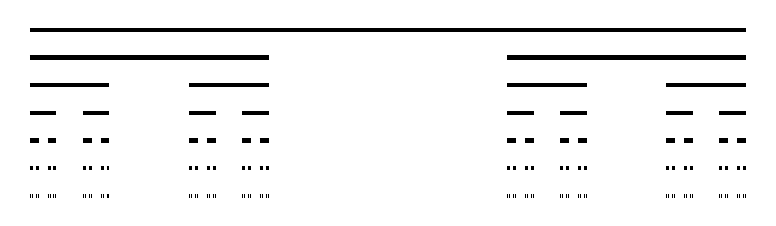
\begin{tikzpicture}
        \foreach \order in {0,...,6}
        \draw[yshift=-\order*10pt, ultra thick]  l-system[l-system={Cantor set, axiom=F, order=\order, step=.75\textwidth/(3^\order)}];
      \end{tikzpicture}
    \end{minipage}%
    \hfill
    \begin{minipage}{.58\textwidth}
      This particular fractal structure is known as the (uniform) \textbf{\alert{Cantor set}}.
      Its dimension is

      \[
      D = \dfrac{\log(2)}{\log(3)} \simeq 0.631
      \]

      \medskip

      It less than a line but more than isolated points.
    \end{minipage}

    \vfill
\end{frame}

\begin{frame}[t, c]{Baker map}{}
  \vfill
  \large

  \begin{minipage}{.38\textwidth}
    \centering
    \includegraphics[width=\textwidth]{Baker_map_5_bis}
  \end{minipage}%
  \hfill
  \begin{minipage}{.58\textwidth}
    \begin{overprint}
      \onslide<1>
      \[
      D = -\lim_{\epsilon \to 0} \dfrac{\log(N)}{\log(\epsilon)}
      \]

      \onslide<2>
      \[
      D = \lim_{n \to \infty} \dfrac{\log \left(2^n \times a^{-n} \right)}{\log \left( a^{-n} \right)}
      \]

      \onslide<3>
      \[
      D = 1 + \dfrac{\log(2)}{\log(\nicefrac{1}{a})}
      \]

      \onslide<4>
      \[
      D \simeq 1.63
      \]
    \end{overprint}
  \end{minipage}

  \vfill
\end{frame}

{
  \setbeamercolor{background canvas}{bg=white}
  \setbeamercolor{background canvas}{bg=white}
  \setbeamercolor{normal text}{fg=black}

  \usebeamercolor[fg]{normal text}

  \setbeamercolor{frametitle}{fg=black}
  \setbeamercolor{framesubtitle}{fg=black}
  \setbeamercolor{itemize item}{fg=black}

  \begin{frame}[fragile]{}{}
    \vfill
    \centering
    \Large
    \textbf{\color{black} Hénon Map}

    \bigskip

    \large
    \textbf{\color{gray} A somewhat analog to Lorenz in discrete-time}
    \vfill
  \end{frame}
}

\begin{frame}[t, c]{Hénon Map (1976)}{}
  \vfill
  \large

  \begin{minipage}{.48\textwidth}
    \[
    \begin{aligned}
      x_{k+1} & = y_k + 1 - \alpha x_k^2 \\
      y_{k+1} & = \beta x_k
    \end{aligned}
    \]
  \end{minipage}%
  \hfill
  \begin{minipage}{.48\textwidth}
    \centering
    \includegraphics[width=.5\textwidth]{henon}

    \bigskip

    \tiny
    Michel Hénon (1931-2013)
  \end{minipage}

  \vfill
\end{frame}

\begin{frame}[t, c]{Hénon Map}{}
  \vfill
  \large
  \centering

  \[
  \begin{aligned}
    x^{\prime} & = x_k \\
    y^{\prime} & = 1 + y_k - \alpha x_k^2
  \end{aligned}
  \]

  \vfill
\end{frame}


\begin{frame}[t, c]{Hénon Map}{}
  \vfill
  \large
  \centering

  \[
  \begin{aligned}
    x^{\prime\prime} & = \beta x^{\prime} \\
    y^{\prime\prime} & = y^{\prime}
  \end{aligned}
  \]

  \vfill
\end{frame}

\begin{frame}[t, c]{Hénon Map}{}
  \vfill
  \large
  \centering

  \[
  \begin{aligned}
    x_{k+1} & = y^{\prime\prime} \\
    y_{k+1} & = x^{\prime\prime}
  \end{aligned}
  \]

  \vfill
\end{frame}

\begin{frame}[t, c]{Hénon Map $(a, b) = (1.4, 0.3)$}{}
  \centering
  \vfill
  \includegraphics[width=.5\textwidth]{Henon_map}
  \vfill
\end{frame}

\begin{frame}[t, c]{Hénon Map $(a, b) = (1.4, 0.3)$}{}
  \centering
  \vfill
  \includegraphics[width=.5\textwidth]{Henon_map_zoom}
  \vfill
\end{frame}


\begin{frame}[t, c]{Hénon Map $(a, b) = (1.4, 0.3)$}{}
  \centering
  \vfill
  \includegraphics[width=.5\textwidth]{Henon_map_zoom_bis}
  \vfill
\end{frame}

{
  \setbeamercolor{background canvas}{bg=white}
  \setbeamercolor{background canvas}{bg=white}
  \setbeamercolor{normal text}{fg=black}

  \usebeamercolor[fg]{normal text}

  \setbeamercolor{frametitle}{fg=black}
  \setbeamercolor{framesubtitle}{fg=black}
  \setbeamercolor{itemize item}{fg=black}

  \begin{frame}[fragile]{}{}
    \vfill
    \centering
    \Large
    \textbf{\color{black} R\"ossler system}

    \bigskip

    \large
    \textbf{\color{gray} Folding and stretching in continuous time}
    \vfill
  \end{frame}
}

\begin{frame}[t, c]{R\"ossler system (1976)}{}
  \vfill
  \large

  \begin{minipage}{.48\textwidth}
    \[
    \begin{aligned}
      \dot{x} & = -y-z \\
      \dot{y} & = x + a y \\
      \dot{z} & = b + z(x-c)
    \end{aligned}
    \]
  \end{minipage}%
  \hfill
  \begin{minipage}{.48\textwidth}
    \centering
    \includegraphics[width=.75\textwidth]{otto_rossler} \\

    \bigskip

    \tiny
    Otto R\"ossler (81 years old)
  \end{minipage}

  \vfill
\end{frame}

\begin{frame}[t, c]{R\"ossler system}{}
  \vfill

  \begin{minipage}{.48\textwidth}
    \centering
    \begin{tikzpicture}
      \begin{axis}[
          width=.8\textwidth,
          hide axis
        ]
        \addplot[smooth, very thin, white] table[x=x, y=y]{data/rossler_orbit_1.dat};
      \end{axis}
    \end{tikzpicture}
  \end{minipage}%
  \hfill
  \begin{minipage}{.48\textwidth}
    \centering
    \begin{tikzpicture}
      \begin{axis}[
          width=.8\textwidth,
          hide axis
        ]
        \addplot[smooth, very thin, white] table[x=x, y=y]{data/rossler_orbit_2.dat};
      \end{axis}
    \end{tikzpicture}
  \end{minipage}

  \vfill

  \begin{minipage}{.48\textwidth}
    \centering
    \begin{tikzpicture}
      \begin{axis}[
          width=.8\textwidth,
          hide axis
        ]
        \addplot[smooth, very thin, white] table[x=x, y=y]{data/rossler_orbit_3.dat};
      \end{axis}
    \end{tikzpicture}
  \end{minipage}%
  \hfill
  \begin{minipage}{.48\textwidth}
    \centering
    \begin{tikzpicture}
      \begin{axis}[
          width=.8\textwidth,
          hide axis
        ]
        \addplot[smooth, very thin, white] table[x=x, y=y]{data/rossler_orbit_4.dat};
      \end{axis}
    \end{tikzpicture}
  \end{minipage}


  \vfill
\end{frame}

{
  \setbeamercolor{background canvas}{bg=white}
  \setbeamercolor{background canvas}{bg=white}
  \setbeamercolor{normal text}{fg=black}

  \usebeamercolor[fg]{normal text}

  \setbeamercolor{frametitle}{fg=black}
  \setbeamercolor{framesubtitle}{fg=black}
  \setbeamercolor{itemize item}{fg=black}

  \begin{frame}[t, c]{R\"ossler system}{}
    \vfill
    \large
    \centering

    \includegraphics[width=.4\textwidth]{rossler_system}

    \vfill
  \end{frame}

  \begin{frame}[t, c]{R\"ossler system}{}
    \vfill
    \large

    \begin{minipage}{.38\textwidth}
      \centering
      \includegraphics[width=\textwidth]{rossler_schematic}
    \end{minipage}%
    \hfill
    \begin{minipage}{.58\textwidth}
      Stretching occurs along the two-dimensional unstable manifold of the spiral-saddle point close to the origin.
    \end{minipage}

    \vfill
  \end{frame}


  \begin{frame}[t, c]{R\"ossler system}{}
    \vfill
    \large

    \begin{minipage}{.38\textwidth}
      \centering
      \includegraphics[width=\textwidth]{rossler_schematic}
    \end{minipage}%
    \hfill
    \begin{minipage}{.58\textwidth}
      Folding and re-injection is induced by along the stable and unstable manifolds of the second fixed point.
    \end{minipage}

    \vfill
  \end{frame}

  \begin{frame}[t, c]{R\"ossler system}{}
    \vfill
    \centering

    \includegraphics[width=.8\textwidth]{rossler_cantor_set}
    \vfill
  \end{frame}

}

{
  \setbeamercolor{background canvas}{bg=white}
  \setbeamercolor{background canvas}{bg=white}
  \setbeamercolor{normal text}{fg=black}

  \usebeamercolor[fg]{normal text}

  \setbeamercolor{frametitle}{fg=black}
  \setbeamercolor{framesubtitle}{fg=black}
  \setbeamercolor{itemize item}{fg=black}

  \begin{frame}
    \vfill
    \Large
    \centering

    \textbf{Four basic mechanisms}

    \bigskip

    \large
    \textbf{\color{gray} Folding, inverted folding, tearing and half-inverted tearing}

    \vfill
  \end{frame}

}

{
  \setbeamercolor{background canvas}{bg=white}
  \setbeamercolor{background canvas}{bg=white}
  \setbeamercolor{normal text}{fg=black}

  \usebeamercolor[fg]{normal text}

  \setbeamercolor{frametitle}{fg=black}
  \setbeamercolor{framesubtitle}{fg=black}
  \setbeamercolor{itemize item}{fg=black}

  \begin{frame}
    \vfill
    \centering
    \large

    \begin{minipage}{.48\textwidth}
      \centering
      \begin{tikzpicture}
        \begin{axis}[
            xmin=-25, xmax=25,
            ymin=0, ymax=50,
            height=.75\textheight,
            hide axis
          ]
          \addplot[smooth, very thin, black, opacity=0.75] table[x=x, y=z]{data/lorenz_attractor.dat};
        \end{axis}
      \end{tikzpicture}
    \end{minipage}%
    \hfill
    \begin{minipage}{.48\textwidth}
      \centering
      \includegraphics[width=.75\textwidth]{rossler_system}
    \end{minipage}

    \vfill
  \end{frame}
}

\begin{frame}[t, c]{Folding}{}
  
\end{frame}

\begin{frame}[t, c]{Inverted folding}{}
  
\end{frame}

\begin{frame}[t, c]{Tearing}{}
  
\end{frame}

\begin{frame}[t, c]{Half-inverted tearing}{}
  
\end{frame}

{
  \setbeamercolor{background canvas}{bg=white}
  \setbeamercolor{background canvas}{bg=white}
  \setbeamercolor{normal text}{fg=black}

  \usebeamercolor[fg]{normal text}

  \setbeamercolor{frametitle}{fg=black}
  \setbeamercolor{framesubtitle}{fg=black}
  \setbeamercolor{itemize item}{fg=black}

  \begin{frame}[fragile]{}{}
    \vfill
    \centering
    \Large
    \textbf{\color{black} What did we not cover in this class ?}

    \vfill
  \end{frame}
}

\begin{frame}
  \vfill
  \large
  \centering

  \textbf{An awful lot !}

  \vfill
\end{frame}

{
  \setbeamercolor{background canvas}{bg=white}
  \setbeamercolor{background canvas}{bg=white}
  \setbeamercolor{normal text}{fg=black}

  \usebeamercolor[fg]{normal text}

  \setbeamercolor{frametitle}{fg=black}
  \setbeamercolor{framesubtitle}{fg=black}
  \setbeamercolor{itemize item}{fg=black}

  \begin{frame}[fragile]{}{}
    \vfill
    \flushright
    \Large
    \textbf{\color{black} Thank you for your attention}

    \large
    \textbf{\color{gray} Any question ?}
    \vfill
  \end{frame}
}

\end{document}
